\subsubsection{Analysis: First Time Mothers of ACT}

\begin{figure}
  \centering
  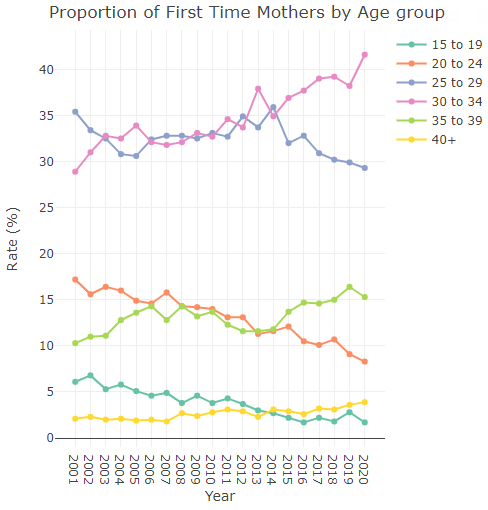
\includegraphics[width=0.5\textwidth]{subsections/age_mothers/first_time_age_group.png}
  \caption{Trends of first-time mother by age group.}
  \label{fig:age2}
\end{figure}

\begin{figure}
  \centering
  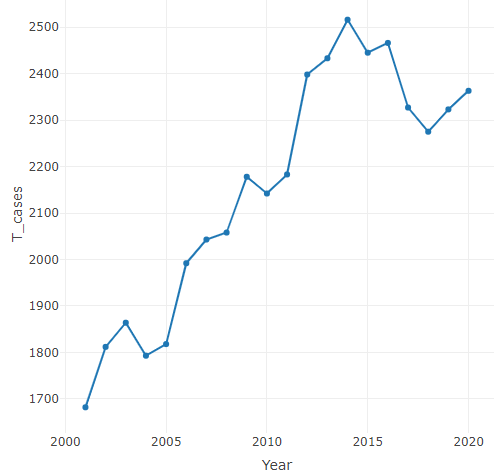
\includegraphics[width=0.45\textwidth]{subsections/age_mothers/first_time.png}
  \caption{Number of first-time mothers in each year.}
  \label{fig:firstTime}
\end{figure}
For a deeper understanding of what we have found in \verb|section 5.2| we were interested to see how many women became mothers for the first time. To achieve that we have generated Figure: \ref{fig:age2} where we can see that although mothers who are aged 40+ tend to have babies less the trend has been changing from the last decade and they have more birthrate than the age group of 15-19 years old. The low birthrate of 15-19 is understandably low as the legal age of consent is 16 except for Tasmania and South Australia which is 17 \cite{consentWebsite}.

Intuitively, this analysis leads us to ask how many women were becoming mothers for the first time each year so that we can observe a trend in women having babies. After generating figure: \ref{fig:firstTime} we can see that number of women becoming first-time mothers has increased over the years.
